% Created 2016-01-10 Sun 17:59
\documentclass[presentation]{beamer}
\usepackage[utf8]{inputenc}
\usepackage[T1]{fontenc}
\usepackage{fixltx2e}
\usepackage{graphicx}
\usepackage{grffile}
\usepackage{longtable}
\usepackage{wrapfig}
\usepackage{rotating}
\usepackage[normalem]{ulem}
\usepackage{amsmath}
\usepackage{textcomp}
\usepackage{amssymb}
\usepackage{capt-of}
\usepackage{hyperref}
\usepackage[activate={true,nocompatibility},final,tracking=true,kerning=true,spacing=true,factor=1100,stretch=10,shrink=10]{microtype}
\usepackage{minted}
\usepackage{svg}
\usepackage[backend=biber,style=alphabetic]{biblatex}
\fvset{fontsize=\footnotesize}
\fvset{frame=lines}
\fvset{framesep=5pt}
\DeclareUnicodeCharacter{200B}{}
\addbibresource{~/Documents/comp3220/master/comp3220.bib}
\AtBeginSection[]{\begin{frame}<beamer>\frametitle{Content}\tableofcontents[currentsection]\end{frame}}
\usetheme{default}
\author{Zhitao Gong}
\date{2016 Spring}
\title{Variable}
\subtitle{COMP3220 -- Principle of Programming Languages}
\hypersetup{
      pdfauthor={Zhitao Gong},
      pdftitle={Variable},
      pdfkeywords={},
      pdfsubject={},
      pdfcreator={Emacs 24.5.1 (Org mode 8.3.2)},
      pdflang={English},
      bookmarks=true,
      unicode=true,
      pdftoolbar=true,
      pdfmenubar=true,
      pdffitwindow=false,
      pdfstartview={FitW},
      pdfnewwindow=true,
      colorlinks=true,
      linkcolor=red,
      citecolor=green,
      filecolor=magenta,
      urlcolor=cyan}
\begin{document}

\maketitle
\begin{frame}{Outline}
\setcounter{tocdepth}{2}
\tableofcontents
\end{frame}


\section{Variable Name}
\label{sec:orgheadline7}

\begin{frame}[label={sec:orgheadline1}]{Variable Name}
A name is a string of characters to identify an entity.  The
following design choices vary in different languages.

\begin{itemize}
\item What characters may be used in names?
\item Case sensitive or not?
\item Special words in the language is reserved words or keywords?
\end{itemize}
\end{frame}

\begin{frame}[fragile,label={sec:orgheadline2}]{Valid Characters}
 \begin{itemize}
\item Most PL allow only ASCII characters, specifically \texttt{[a-zA-Z0-9\_]}.
\item Some allow certain Unicode characters, e.g., \texttt{C\#}. \texttt{Java}.

\begin{figure}[htb]
\centering
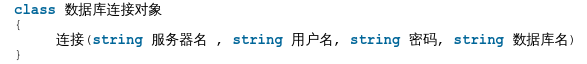
\includegraphics[width=.9\linewidth]{img/csharp-unicode.png}
\caption{\texttt{C\#} class with Chinese Characters LOL}
\end{figure}

\item Character set isn’t the problem.  The non-descriptive, one-letter
identifiers are.
\end{itemize}
\end{frame}

\begin{frame}[fragile,label={sec:orgheadline3}]{\texttt{C++} Convention}
 \begin{minted}[]{cpp}
int main() {
  int sum;                      // good
  int v1, vv;                   // OK, but meaningless
  int ____v2, v3_____, _;       // OK, but NEVER DO THIS
  int 2v;                       // WRONG
}
\end{minted}

\begin{quote}
never use "underhanded names," ones that begin with an underscore
or that contain a double underscore (p2 , C++ Coding Standards,
Herb Sutter and Andrei Alexandrescu)
\end{quote}

\begin{itemize}
\item Names beginning with an underscore or a double underscore are
RESERVED for the C++ implementers.
\item Names with an underscore are reserved for the library to work.
\end{itemize}
\end{frame}

\begin{frame}[fragile,label={sec:orgheadline4}]{\texttt{C++} Naming Style}
 \begin{description}
\item[{CamelCase}] In Compound words or phrases, each word or
abbreviation begins with a capital letter, e.g.,
\texttt{UpperCamelCase} or \texttt{lowerCamelCase}.
\item[{snake\_case}] Words are separated with one underscore character
(\_) and no spaces, with each element's initial letter usually
lowercased.
\end{description}
\end{frame}

\begin{frame}[fragile,label={sec:orgheadline5}]{Special Words}
 Special words in programming languages are used to make programs
more readable by naming actions to be performed.

\begin{description}
\item[{Keyword}] A word of a programming language that is special only
in certain contexts, a part of the syntax, e.g., FORTRAN.

\begin{minted}[]{fortran}
Integer Apple
Integer = 4
Integer Real
Real Integer
\end{minted}

\item[{Reserved Word}] A special word of a programming language that
\emph{cannot} be used as a name.  It is always a better choice
unless too many words are reserved, e.g., \texttt{COBOL}.
\end{description}
\end{frame}

\begin{frame}[fragile,label={sec:orgheadline6}]{Special Words Cont'd}
 In practice \emph{most} keywords are reserved words and vice versa.

\begin{itemize}
\item Keyword may not be a reserved word, e.g. a keyword only has
meaning in a special context, and may be used as an identifier.
E.g., in Fortran, we may have

\begin{minted}[]{fortran}
 IF (if) THEN
    then
 ELSE
    else
 END IF
\end{minted}

\item Reserved word may not be keyword, e.g. reserved for future use.
E.g., \texttt{goto} in \texttt{Java}.
\end{itemize}
\end{frame}

\section{Address and Value}
\label{sec:orgheadline14}

\begin{frame}[label={sec:orgheadline8}]{Address of Variable}
\begin{description}
\item[{Address of a variable}] The machine memory address with which it
is associated.
\end{description}


\begin{itemize}
\item The same variable name may be associated with different addresses
at different times in the program
\item Multiple variables name may refer to the same memory location.
\end{itemize}


The address of a variable is sometimes called its L-value, since it
appears on the left-hand side of an assignment.
\end{frame}

\begin{frame}[fragile,label={sec:orgheadline9}]{One Variable Bound to Multiple Addresses}
 \begin{minted}[]{cpp}
void foo() {
  int a = 3;
}

int main() {
  foo();
  foo();
}
\end{minted}

Variable \texttt{a} is created on the \emph{runtime stack}.  Different calls of
\texttt{foo()} may result in the local variable \texttt{a} bound to different
addresses.
\end{frame}

\begin{frame}[fragile,label={sec:orgheadline10}]{Multiple Variables Bound to Same Address}
 These variables are \emph{aliases}.

\begin{itemize}
\item Aliasing is a hindrance to readability.
\item It is error-prone.
\item However, alias is sometimes preferred.
\end{itemize}


\begin{minted}[]{cpp}
void foo(int& v) {
  v += 2;
}
int main() {
  int a = 3;
  foo(a);  // value of a after this call?
  int& b = a;
  b += 3;  // value of a after this statement?
}
\end{minted}
\end{frame}

\begin{frame}[fragile,label={sec:orgheadline11}]{\texttt{C++} Alias Problem}
 The following code causes problems because of aliases.

\begin{minted}[]{cpp}
int main() {
  int* a = new int{3};
  int* b = a;

  *b = 100;  // value of a after this statement?
  delete a;  // what about b?
  delete b;  // ERROR
}
\end{minted}

We will revisit the \emph{dangling pointer} problem.
\end{frame}

\begin{frame}[fragile,label={sec:orgheadline12}]{\texttt{C++} Alias Advantage}
 If we have a big user-defined types, e.g., \texttt{class C}.  Pass it by
value to a function call may be too space and time consuming.

\begin{minted}[]{cpp}
class C {
  // a big class
};
void foo(const C& c) {
  // awesome function
}
int main() {
  C c;
  foo(c);
}
\end{minted}

In this case, an alias is preferred.
\end{frame}

\begin{frame}[fragile,label={sec:orgheadline13}]{Value}
 \begin{description}
\item[{Value of a variable}] The contents of the memory cell or cells
associated with the variable.  A variable's value is sometimes
called its R-value.
\end{description}


\begin{minted}[]{cpp}
int main() {
  int a = 3;
  int b = a + 3;
  b + 4 = 4  // ERROR!
}
\end{minted}
\end{frame}

\section{Binding}
\label{sec:orgheadline21}

\begin{frame}[fragile,label={sec:orgheadline15}]{Concept of Binding}
 \begin{description}
\item[{Binding}] An association between an attribute, e.g., name, type,
value, address and etc., and an entity, e.g., an identifier or
a symbol.
\end{description}

Some binding examples

\begin{itemize}
\item The meaning of reserved words \texttt{if}.
\item The operation associated with a symbol \texttt{*}.
\item The entity (variable, keyword, etc.) represented by an identifier.
\item The range of data type, e.g., \texttt{int}.
\item etc.
\end{itemize}
\end{frame}

\begin{frame}[fragile,label={sec:orgheadline16}]{Binding Time}
 The time when a binding occurs is called \emph{binding time}.  Common
binding times include (in chronological order):

\begin{itemize}
\item Language definition, e.g, general meaning of \texttt{+}
\item Language implementation, e.g., internal representation of 23
\item \emph{Program translation (compile time)}, e.g., data type
\item Link edit, e.g., a function call to a library
\item Load, e.g., variable storage binding
\item \emph{Program execution (run time)}, e.g., value.
\end{itemize}
\end{frame}

\begin{frame}[fragile,label={sec:orgheadline17}]{Name Binding}
 In most PL's, programmers may bind a name, \emph{identifiers}, to
program entities, e.g., variables, constants, functions, data
types, and etc.

\begin{description}
\item[{Name Binding}] Find the corresponding binding occurrence
(definition/declaration) for an applied occurrence (usage) of
an identifier.
\end{description}


\begin{minted}[]{cpp}
#include <iostream>
using namespace std;

int main() {
  int b = 3;
  {
    int b = 4;
    cout << b << endl;
  }
  cout << b << endl;
}
\end{minted}
\end{frame}

\begin{frame}[fragile,label={sec:orgheadline18}]{Static Type Binding}
 In both cases, the type of a variable cannot change.

\begin{description}
\item[{Explicit Declaration}] Lists variable names and specifies that
they are a particular type.
\end{description}


\begin{minted}[]{cpp}
int main() {
  int a = 3;
}
\end{minted}

\begin{description}
\item[{Implicit Declaration}] Associating variables with types through
default conventions.  E.g., in \texttt{FORTRAN}, variables prefixed
with \texttt{I}, \texttt{J}, \texttt{K}, \texttt{L}, \texttt{M}, \texttt{N} or their lowercase versions
are \emph{implicitly} \texttt{Integer}, otherwise \texttt{Real}.
\end{description}


\begin{minted}[]{cpp}
int main() {
  auto a = 3.3;  // type deduction in C++11
}
\end{minted}
\end{frame}

\begin{frame}[fragile,label={sec:orgheadline19}]{\texttt{C++} Type Deduction}
 \begin{minted}[]{cpp}
#include <iostream>
#include <cmath>
#include <typeinfo>

// same as: double (*get_fun())(double)
auto get_fun() -> double (*)(double)
{
  return std::sin;
}
int main() {
  auto fun = get_fun();
  std::cout << "type of my_fun: " << typeid(fun).name() << '\n';
  std::cout << "fun: " << fun(3) << '\n';
}
\end{minted}

You will see the type "PFddE" which is \texttt{GCC} mangled name.
\texttt{c++filt -t PFddE} returns \texttt{double (*)(double)}.
\end{frame}

\begin{frame}[fragile,label={sec:orgheadline20}]{Dynamic Type Binding}
 Variable type is determined by "assignment".  Usually found in
script languages, \texttt{Javascript}, \texttt{Python}, \texttt{Lua}, etc.

\begin{minted}[]{js}
var a = 3;
a = [1, 2];
a = "A String";
a = {"hello": 1, "world": 3};
\end{minted}

Disadvantages include
\begin{itemize}
\item Code is less reliable.
\item Dynamic binding cost is high.
\item Type checking must be done at run time.
\item Space for Run-time type descriptor.
\end{itemize}
\end{frame}

\section{Scope and Lifetime}
\label{sec:orgheadline41}

\begin{frame}[fragile,label={sec:orgheadline22}]{Scope}
 \begin{description}
\item[{Scope of a Variable}] The range of statements in which the
variable is visible. i.e., it can be referenced in that
statement.
\end{description}


\begin{minted}[]{cpp}
#include <iostream>
using namespace std;

int main() {
  int a = 3;
  for (int i = 0; i < 10; ++i) {
    a += i;
  }
  cout << a << endl;
  cout << i << endl;  // ERROR
}
\end{minted}
\end{frame}

\begin{frame}[fragile,label={sec:orgheadline23}]{Reference Environment}
 \begin{description}
\item[{Referencing Environment (RE)}] The collection of all variables
that are visible in the statement.
\end{description}


\begin{minted}[]{cpp}
int g = 3;

int main() {
  // RE: global g

  int a{3}, b{4};
  for (int i = 0; i < 10; ++i) {
    // RE: global g and local a, b, i
  }

  // RE: global g and local a, b

  // Why global g is accessible?
}
\end{minted}
\end{frame}

\begin{frame}[fragile,label={sec:orgheadline24}]{Local Scope}
 Visible within function or statement block from point of
declaration until the end of the block.

\begin{minted}[]{cpp}
void foo(int n) {
  int a = 3;
}

int main() {
  int a = 3;
  for (int i = 0; i < 3; ++i) {
    int b;
  }
}
\end{minted}
\end{frame}

\begin{frame}[fragile,label={sec:orgheadline25}]{Class Scope}
 Visible in class members.  \texttt{a\_} is declared in the \texttt{private}
section of class \texttt{C}, and is accessible within the definition of
the class.

\begin{minted}[]{cpp}
class C {
 public:
  C() : a_(4) {  }

  int get_a() const { return a_; }
  void set_a(int a) { a_ = a; }
 private:
  int a_;
};  // REMEMBER Semicolon!!!

int main() {
  C c1;
  C c2;
}
\end{minted}
\end{frame}

\begin{frame}[fragile,label={sec:orgheadline26}]{Namespace Scope}
 Visible within same namespace block.

\begin{minted}[]{cpp}
namespace foo {
int a;
}

void f1() {
  a = 3;  // ERROR
}

namespace foo {
void f2() {
  a = 4;  // OK
}}

int main() {
  a = 3;      // ERROR
  foo::a = 3; // OK
}
\end{minted}
\end{frame}

\begin{frame}[fragile,label={sec:orgheadline27}]{File Scope}
 Visible within current file.

\begin{columns}
\begin{column}{0.5\columnwidth}
\begin{block}{Foo}
\begin{minted}[]{cpp}
// foo.cpp
#include "foo.h"
int pub_var;
static int pri_var;

void foo()
{
  pub_var = 1;
  pri_var = 2;
}
\end{minted}

\begin{minted}[]{cpp}
// foo.h
void foo();
\end{minted}
\end{block}
\end{column}

\begin{column}{0.5\columnwidth}
\begin{block}{Main}
\begin{minted}[]{cpp}
#include <iostream>
#include "foo.h"
using namespace std;

int main() {
  extern int pub_var;
  extern int pri_var;
  foo();
  cout << pub_var << endl  // OK
       << pri_var << endl; // ERROR
}
\end{minted}

Compile with \texttt{g++ main.cpp foo.cpp}.
\end{block}
\end{column}
\end{columns}
\end{frame}

\begin{frame}[fragile,label={sec:orgheadline28}]{Global Scope}
 Visible everywhere unless \emph{shadowed}.

\begin{minted}[]{cpp}
int g = 3;

int main() {
  g = 3;
  int g = 4;
  ::g = 33;
}
\end{minted}

Different from file scope: \texttt{static} prefix.
\end{frame}

\begin{frame}[fragile,label={sec:orgheadline29}]{Scope Rule}
 Scope rules of a PL determine how a particular occurrence of a name
is associated with a variable.  Implicitly, variable are visible
inside there declaration block, i.e., \emph{local scope}.

\begin{minted}[]{cpp}
int a = 3;

int main() {
  a = 4;
  int a = 100;
}
\end{minted}

In particular, scope rules determine how references to variables
declared \emph{outside} the currently executing subprogram or block are
associated with their declarations and thus their attributes.
\end{frame}

\begin{frame}[fragile,label={sec:orgheadline30}]{Static/Lexical Scoping}
 Bind a name to a non-local variable at \emph{compile time}.  Find the
smallest block syntactically enclosing the reference and containing
a declaration of the variable.

\begin{minted}[]{cpp}
#include <iostream>
using namespace std;
int b = 0;
int foo() {
  int a = b + 1;  // b is NOT declared inside foo
  return a;
}
int bar() {
  int b = 1;
  return foo();
}
int main() {
  cout << foo() << endl;
  cout << bar() << endl;
}
\end{minted}
\end{frame}

\begin{frame}[fragile,label={sec:orgheadline31}]{Nested Static Scoping}
 Two categories of static scoping: subprograms may be nested (nested
static scoping) and those may not be nested.

\begin{minted}[]{js}
function fun1() {
  var v1 = 3;                   // v1 in fun1

  function fun2() {             // fun2 defined in fun1
    var v1 = 3;                 // v1 in fun2
    fun3();
  }

  function fun3() {             // fun3 defined in fun1
    console.log(v1);            // which v1 to use?
  }

  fun2();
}
\end{minted}
\end{frame}

\begin{frame}[fragile,label={sec:orgheadline32}]{Dynamic Scoping}
 Bind a name to a non-local variable at \emph{run time}.  Find the most
recent, currently active run-time stack frame containing a
declaration of the variable.

\begin{minted}[]{cpp}
#include <iostream>
using namespace std;
int b = 0;
int foo() {
  int a = b + 1;  // b is NOT declared inside foo
  return a;
}
int bar() {
  int b = 1;
  return foo();
}
int main() {
  cout << foo() << endl;
  cout << bar() << endl;
}
\end{minted}
\end{frame}

\begin{frame}[fragile,label={sec:orgheadline33}]{Nested Dynamic Scoping}
 Suppose the following program uses dynamic scoping.

\begin{minted}[]{js}
function fun1() {
  var v1 = 1;                   // v1 in fun1

  function fun2() {             // fun2 defined in fun1
    var v1 = -1;                // v1 in fun2
    fun3();
  }

  function fun3() {             // fun3 defined in fun1
    console.log(v1);            // which v1 to use?
  }

  fun2();
}
\end{minted}
\end{frame}

\begin{frame}[fragile,label={sec:orgheadline34}]{Problem -- Static Scoping}
 Code refining may break the program.  Solution?  Global variable or
modularization/encapsulation.

\begin{columns}
\begin{column}{0.5\columnwidth}
\begin{minted}[]{js}
function fun1() {
  var v1 = 1;

  function fun2() {
    var v1 = -1;
    fun3();
  }

  function fun3() {
    console.log(v1);
  }

  fun2();
}
\end{minted}
\end{column}

\begin{column}{0.5\columnwidth}
\begin{minted}[]{js}
function fun1() {
  var v1 = 1;

  function fun2() {
    var v1 = -1;

    function fun3() {
      console.log(v1);
    }
    fun3();
  }

  fun2();
}
\end{minted}
\end{column}
\end{columns}
\end{frame}

\begin{frame}[label={sec:orgheadline35}]{Problem -- Dynamic Scoping}
\begin{itemize}
\item Programs hard to read and understand.
\begin{itemize}
\item The correct attributes (e.g., values) of non-local variables
cannot be determined statically (e.g., by reading).
\item Reference to the name of a variable is not always to the same
variable.
\end{itemize}
\item Type checking for non-local variables.
\item Access to non-local variable is generally slower.
\end{itemize}
\end{frame}

\begin{frame}[label={sec:orgheadline36}]{Lifetime}
\begin{description}
\item[{Lifetime of a variable}] The time period in which the object has
valid memory, i.e., the period during execution of a program
in which a variable or function exists.  The \emph{storage
duration} of the identifier determines its lifetime.
\end{description}


Generall speaking

\[\text{Lifetime}\geq \text{Scope}
   \]
\end{frame}

\begin{frame}[fragile,label={sec:orgheadline37}]{Static Variable Lifetime}
 A \emph{static variable} is stored in the \emph{data segment} of the "object
file" of a program.  Its lifetime is the entire duration of the
program's execution.

\begin{minted}[]{cpp}
#include <iostream>
using namespace std;

int foo() {
  static int a = 0;
  a++;
  return a;
}

int main() {
  cout << foo() << endl;  // output?
  cout << foo() << endl;  // output?
}
\end{minted}
\end{frame}

\begin{frame}[fragile,label={sec:orgheadline38}]{Automatic Variable Lifetime}
 \begin{itemize}
\item Begins when program execution enters the function or statement block or compound and
\item ends when execution leaves the block.
\end{itemize}


Automatic variables are stored on a "function call stack".

\begin{minted}[]{cpp}
#include <iostream>
using namespace std;

int foo() {
  int a = 0;
  ++a;
  return a;
}

int main() {
  cout << foo() << endl;  // output?
  cout << foo() << endl;  // output?
}
\end{minted}
\end{frame}

\begin{frame}[fragile,label={sec:orgheadline39}]{Dynamic Variable Lifetime}
 \begin{itemize}
\item Begins when memory is allocated for the object and
\item ends when memory is deallocated.
\end{itemize}


Dynamic objects are stored on "the heap".

\begin{minted}[]{cpp}
#include <iostream>
using namespace std;

int foo() {
  int* a = new int{3};
  int* b = new int{3};
  ++(*a);
  delete b;
  return *a;
}
int main() {
  cout << foo() << endl;  // output?
  cout << foo() << endl;  // output?
}
\end{minted}
\end{frame}

\begin{frame}[fragile,label={sec:orgheadline40}]{Declaration vs Definition}
 \begin{description}
\item[{Declaration}] Tells the compiler the type of a variable, object
or function.
\item[{Definition}] Allocates memory for a variable or object or
implement the details of a function.
\end{description}


Multiple declarations are allowed, but only one definition.

\begin{minted}[]{cpp}
void foo();  // declaration of foo
int main() {
  int a;         // declaration of a;
  a = 3;         // definition of a
}

void foo() { }  // definition of foo
\end{minted}
\end{frame}

\section{Summary}
\label{sec:orgheadline43}

\begin{frame}[label={sec:orgheadline42}]{Summary}
\begin{itemize}
\item Variable names, naming styles
\item Variable Scope and lifetime.
\end{itemize}
\end{frame}
\end{document}
